\documentclass{article}
\usepackage{listings}
\usepackage{graphicx}
\graphicspath{ {/} }
\begin{document}
\begin{titlepage}
\centering

{\bfseries\LARGE Instituto Polit\'ecnico Nacional \par}
\vspace{1cm}
{\scshape\Large Escuela Superiror de Computaci\'on \par}
\vspace{3cm}
{\scshape\Large Teoria de la Computaci\'on \par}
\vspace{3cm}
{\itshape\Large Pr\'actica 1 \par}
{\itshape\Large Universo \par}
\vfill
{\Large Profesor: \par}
{\Large Genaro Juarez Martinez \par}
{\Large Alumno: \par}
{\Large Alcantara Covarrubias Erik \par}
{\Large Email: erik.alcova@gmail.com \par}
{\Large Grupo: 4SCM6\par}
\vfill
\end{titlepage}

\tableofcontents

\newpage

\section{Introducción}
La base de los automatas, que es el tema central de estudio del primer parcial de la materia, es el poder hablar de lenguajes. Cada ser humano ocupa un lenguaje como el español o el ingles. 
\\Pero los automatas ocupan una definicion diferente para un lenguaje:
\begin{itemize}
    \item Un lenguaje se conforma por un alfabeto.
    \item Un alfabeto es un numero finito de simbolos que tienen un significado.
\end{itemize}

\section{Marco Teorico}

\begin{itemize}
    \item Lenguaje ($\sum$): Conjunto de simbolos que conforman un alfabeto
    \\$\sum = \{ 0, 1\}$ Es un lenguaje conformado por el 0 y el 1.
    \\$\sum = \{A, ..., Z\}$ Es un lenguaje conformado por las letras arabigas.\\
    \item Potencia de un Alfabeto ($\sum^n$): Con esta notacion podemos decir cuantas cadenas de n largo se pueden formulario
    \\$\sum = \{0,1\}$
    \\$\sum^0 = \{\epsilon\}$
    \\$\sum^1 = \{0,1\}$
    \\$\sum^2 = \{00,01,10,11\}$
    \\$\sum^n = \{...\}$\\
    \\Nota: $\sum ^*$ es lo mismo que la union de todas las potencias.
    \\\\$\sum ^*$=$\sum^0\bigcup\sum^1\bigcup\sum^2\bigcup...\bigcup\sum^n$
    \item String: Es una cadena de simbolos finita\\
    \item Cadena vacia $\{\epsilon \}$: Es el string que no contiene ningun elemento\\
    \item Longitud de una string $|abc... \vert $ : Es la cantidad de simbolos que tiene un string\\
    \item Lenguaje(\emph{L}):Es el conjunto de todas las cadenas posibles de nuestro alfabeto.
    \\$\emph{L}\subseteq(\sum)^*$
    \item Permutas ($n!$): Cuando un algoritmo tiene un coste factorial es prácticamente inutilizable para valores no muy
    grandes. Es evidente que $n!$ es extremadamente costoso con respecto a los otros.
    \\$1! = 1$, $2! = 2$, $3! = 6$, $4! = 24$
    
\end{itemize}

\section{Desarrollo}

\subsection{Programa 1 - Universo}
Programar el universo de las cadenas binarias $(\Sigma^n)$. Dada una "n" que introduzca el usuario o que el programa lo determine automáticamente.
\\El rango de "n" debe de estar en el intervalo de [0, 1000].
\begin{enumerate}
    \item El programa debe de preguntar si quiere calcular otra "n" o no y salir hasta que se le especifique.
    \item La salida debe ser expresada en notación de conjunto y debe ir a un archivo de texto.
    \item Del archivo de salida calculado, graficar el número símbolos de cada cadena y otra gráfica de 1s de cada cadena. El eje de las "x" representan el número de cadenas y el eje de las "y" el número de símbolos que tiene cada cadena. 
    \\Al mismo tiempo calcular el logaritmo base 10 de esas dos gráficas, en total serán cuatro gráficas.
\end{enumerate} 

\subsection{Planteamiento}
Lo mas facil, desde un punto de vista de un programador, es sacar todas las combinaciones posibles de 0 y 1, para despues calcular que tantos 1 tiene cada nueva n y que tantos digitos tienen.
\\Con esto ya tendriamos la mayoria de la logica que se va a usar en el programa, que en este caso esta escrito en python3. 
\\Ya que tiene varias bibliotecas que facilitan mucho la ejecucion de los requerimientos antes señalados.

\subsection{Codigo}

\begin{lstlisting}
    #Declaracion de todas las bibliotecas
    import random
    import matplotlib.pyplot as plt
    import itertools
    import time
    import math
    
    def ingerir(unos, largo):
        """Crea las graficas necesarias"""
        
        graficar(unos, "2^n", "# de unos")
        graficar(largo, "2^n", "# de digitos")
        graficar(logrec(unos), "2^n", "log10(# de unos)")
        graficar(logrec(largo), "2^n", "log10(# de digitos)")
        
    def logrec(array):
        """Aplica log base 10 a cada elemento del array"""
        aux=[]
        for i in array:
            aux.append(math.log10(int(i)))
        return aux
    
    def graficar(y_axis, titlex, titley):
        """Funcion que genera las graficas"""
        try:
            inicio = time.time()
            ax = plt.subplot()
            plt.xlabel(titlex)
            plt.ylabel(titley)
            plt.title(titlex + " y "+titley)
            ax.plot(y_axis)
            fin = time.time()
            plt.show()
            print("El tiempo de ejecucion para la grafica: "+titlex+", "+titley+" es: "+str(fin-inicio))
            plt.savefig(titlex+titley+".png")
            
        except (KeyboardInterrupt, BufferError):
            fin = time.time()
            plt.show()
            print("El tiempo de ejecucion para la grafica: "+titlex+", "+titley+" es: "+str(fin-inicio))
        
    def permutaciones(bit):
        """Crea todas las permutaciones posibles"""
        
        in_file=open("Practica1/permutaciones.txt", "w")
        in_file.write("L{e\n")
        inicio = time.time()
        i = 0
        num_unos = []
        num_digitos = []
        
        while(i < bit):
            
            liminf = 2**i
            limsup = (2**(i+1))
            limmed = math.floor(limsup/4)
            unos = 0
            
            try:
                subsets = list(itertools.islice(itertools.product(*[[0,1]]*(i+1)), liminf, limmed))
                in_file.write(","+' '.join(map(str, subsets)))
                unos += sum(map(sum, subsets))
                #print(subsets)
                del subsets
                
                subsets = list(itertools.islice(itertools.product(*[[0,1]]*(i+1)), limmed, (limmed*2)))
                in_file.write(' '.join(map(str, subsets)))
                unos += sum(map(sum, subsets))
                #print(subsets)
                del subsets
                
                subsets = list(itertools.islice(itertools.product(*[[0,1]]*(i+1)), (limmed*2), (limmed*3)))
                in_file.write(' '.join(map(str, subsets)))
                unos += sum(map(sum, subsets))
                #print(subsets)
                del subsets
                
                subsets = list(itertools.islice(itertools.product(*[[0,1]]*(i+1)), (limmed*3), limsup))
                in_file.write(' '.join(map(str, subsets))+"\n")
                unos += sum(map(sum, subsets))
                #print(subsets)
                del subsets
                
                i += 1
                num_unos.append(unos)  
                num_digitos.append(i)     
                del unos
                
            except (KeyboardInterrupt,OverflowError):
                break
        
        in_file.write("}")
        in_file.close()
        print(num_unos)
        
        fin = time.time()
        
        print("El tiempo de ejecucion es: "+str(fin-inicio))
        ingerir(num_unos, num_digitos)
            
                
    if __name__ == "__main__":
        """funcion principal"""
        
        while True:
            print("\nMENU")
            print("1) Modo manual")
            print("2) Modo automatico")
            print("3) Salir")
            aux = int(input("Seleccione una opcion: "))
                
            if aux == 1:
                n = int(input("\nIntroduce n, no mayor a 1000 ni menor a 0: "))
                if 100 < n < 0:
                    print("Error, el numero introducido no es valido")
                    break
                permutaciones(n)
            elif aux ==2:
                n = random.randrange(2,2e7)
                permutaciones(n)
                
            elif aux == 3:
                exit()    
            
            else:
                print("Error, seleccione una opcion correcta")
                break
\end{lstlisting}

\section{Resultados}

Los siguientes son los resultados obtenidos al correr el programa con $n = 27$:
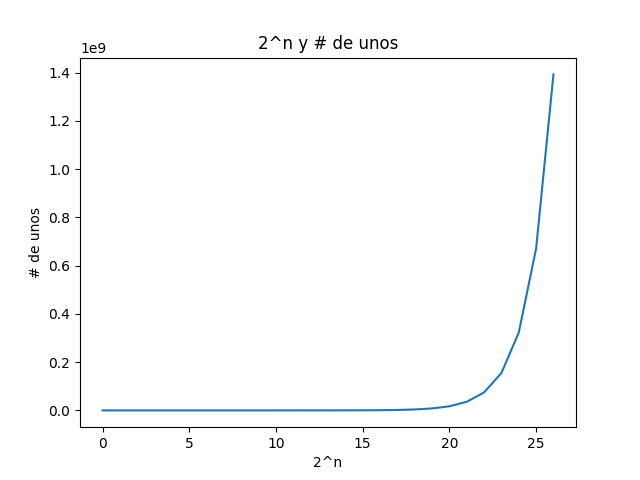
\includegraphics{Graph1.png}
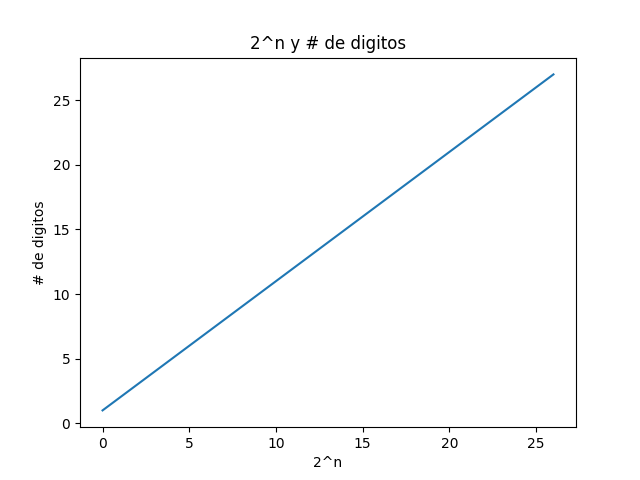
\includegraphics{Graph2.png}
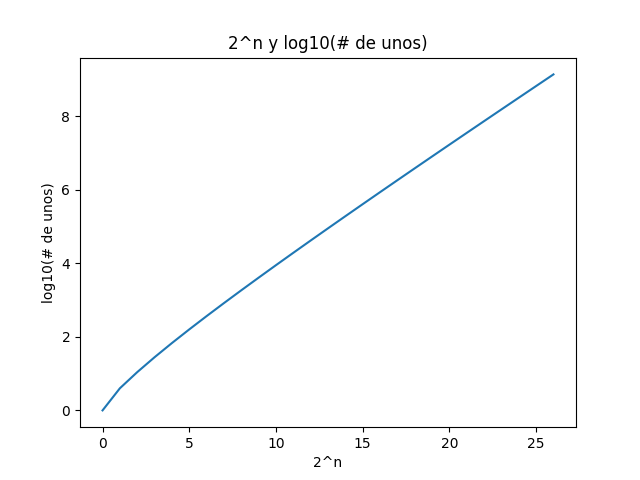
\includegraphics{Graph3.png}
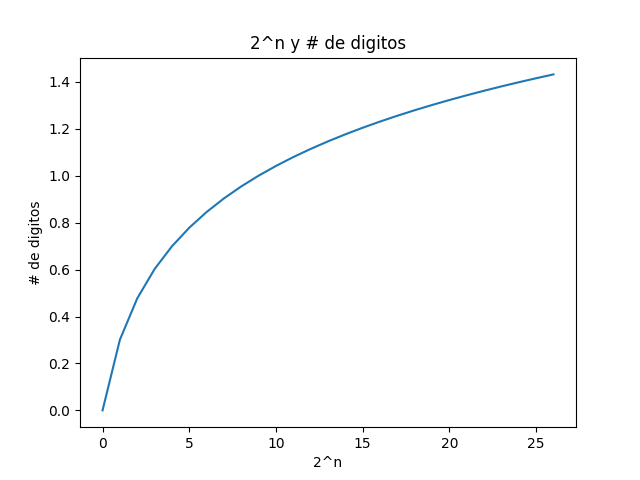
\includegraphics{Graph4.png}
Tambien se creo un archivo .txt que contiene todas las permutaciones sin embargo pesa 14gb por lo que no se puede incluir en los extras de este programa.\\
\\Nota: En la ultima grafica se deben de mostrar los $log_{10}$(num de digitos) pero no se puso en el titulo, sin embargo es correcta la representacion
\\ 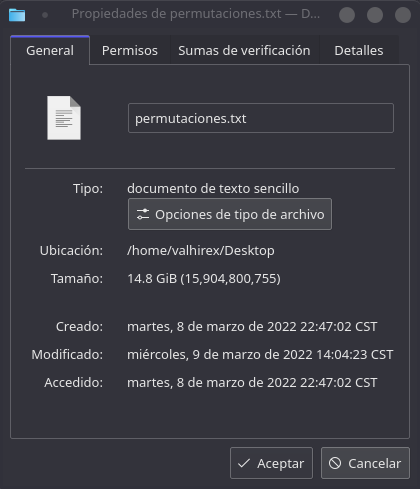
\includegraphics{Archivo.png}

\section{Conclusión}
Este algoritmo pone a prueba los conocimientos en programacion del programador, definitivamente se necesitan conocimientos de un lenguaje de programacion, si no, de todo tu conocimiento tecnico.
\\El programa puede ser mas optimizado incluso si se divide en 2 lenguajes podria reducirse su tiempo de ejecucion mucho mas, pero en el transcurso de realizarlo pasamos de poder ejecutarlo en 6h a unos 5-6 minutos con $n=27$
\\Con esta pudimos aprender la importancia de optimizar el codigo o incluso de mejorar la logica de cada instruccion para mejorar la rapidez.

\section{Referencias bibliograficas}
\begin{itemize}
    \item LaTeX - A document preparation system. (s. f.). LaTeX - A document preparation system. https://www.latex-project.org/
    \item itertools - Biblioteca para hacer iteraciones. https://docs.python.org/3/library/itertools.html
\end{itemize}
\end{document}